%%%%%%%%%%%%%%%%%%%%%%%%%%%%%%%%%%%%%%%%%%%%%%%%%%%%%%%%%%%%%%%%%%%%%%%%%%%%%%%%%%%%%
%																					%
%	TRABAJO: Proyecto Integrador													%
%																					%
%		Titulo: 	Desarrollo de IP cores con procesamiento de Redes de Petri 		%
%					Temporales para sistemas multicore en FPGA						%
%																					%
%		Autores:	Juli�n Nonino													%
%					Carlos Renzo Pisetta											%
%		Director:	Orlando Micolini												%
%																					%
%	Parte: Apendices																%
%	Capitulo: Nuevo proyecto en Xilinx XPS											%
%	Archivo: nuevos_proyectos_XPS.tex												%
%																					%
%%%%%%%%%%%%%%%%%%%%%%%%%%%%%%%%%%%%%%%%%%%%%%%%%%%%%%%%%%%%%%%%%%%%%%%%%%%%%%%%%%%%%

% Path Imagenes: ./apendices/nuevos_proyectos_XPS/img
% Nombre predeterminado imagenes: proyectoxx
%	xx es el numero de imagen

\chapter{Nuevo proyecto en Xilinx XPS}
	\label{ap:nuevos_proyectos_XPS}

	La creaci�n de un nuevo proyecto con procesadores MicroBlaze utilizando la herramienta \emph{Xilinx Platform Studio (XPS)}
	\cite{xilinx_edk} es sencilla.
	
	Para comenzar, esta es la ventana principal de la herramienta.
	\begin{figure}[H]
		\centering
		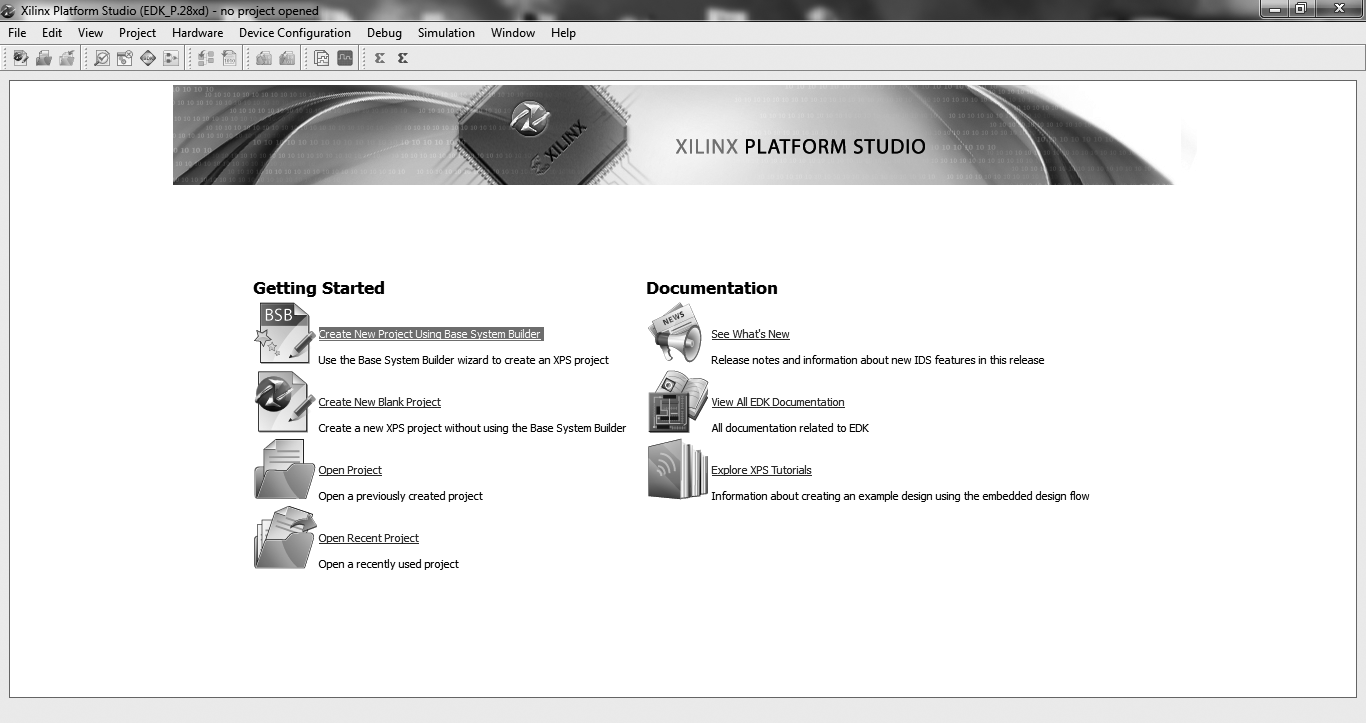
\includegraphics[width=0.7\linewidth,keepaspectratio]{./apendices/nuevos_proyectos_XPS/img/proyecto01}
		\caption{Ventana principal de la herramienta Xilinx Platform Studio}
		\label{fig:proyecto01}
	\end{figure}
	En ella se observan las posibilidades que existen para comenzar a trabajar con un proyecto, abrir uno ya existente, 
	crear un nuevo proyecto en blanco o utilizar el asistente con \textbf{\emph{Base System Builder}} que genera todo 
	el entorno necesario para un determinado kit de desarrollo. Esa es la opci�n que se seguir� en este ap�ndice.
	Al seleccionar �sta opci�n aparecer� una nueva ventana donde se podr� seleccionar:
	\begin{itemize}
	  	\item La ubicaci�n del proyecto.
	  	\item Si el sistema estar interconectado con el bus PLB o con el bus AXI.
	  	\item Si se desean cargar las opciones del sistema desde un archivo ya existente.
	  	\item Si existe alg�n repositorio de perif�ricos espec�ficos para la plataforma que se desea utilizar. En este 
	  		caso, se introducir� un camino hacia IP cores especiales para el kit Digilent Atlys descargados desde el 
	  		sitio del fabricante.
	\end{itemize}
	
	\newpage
		
	\begin{figure}[H]
		\centering
		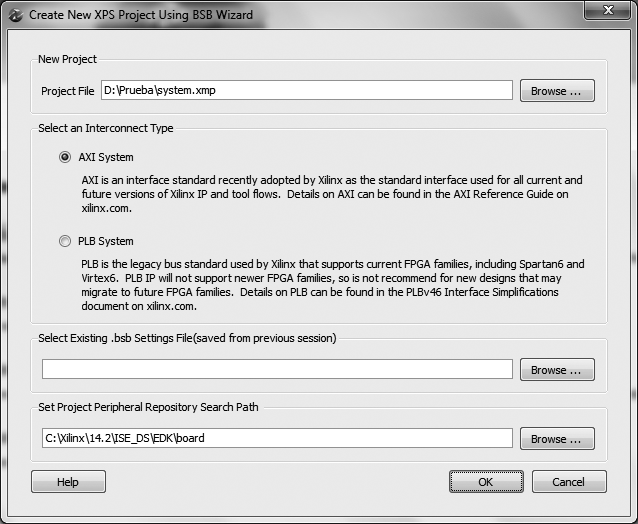
\includegraphics[width=0.6\linewidth,keepaspectratio]{./apendices/nuevos_proyectos_XPS/img/proyecto03}
		\caption{Ventana principal de asistente de creaci�n de proyectos del XPS}
		\label{fig:proyecto03}
	\end{figure}
	
	Luego, al hacer click en \emph{OK} se abrir� la siguiente ventana del asistente que guiar� el proceso de configuraci�n 
	del sistema y del MicroBlaze.
	
	\begin{figure}[H]
		\centering
		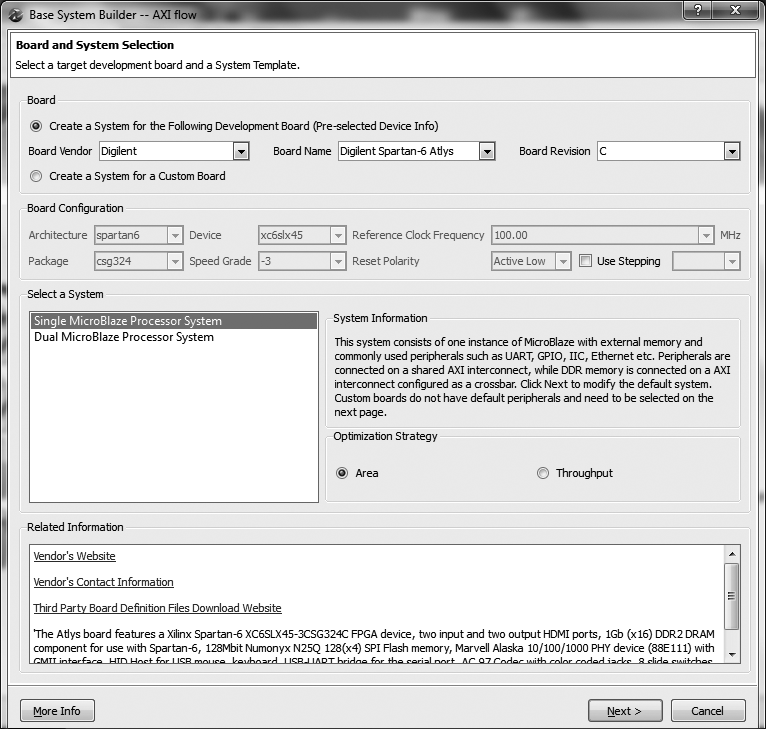
\includegraphics[width=0.6\linewidth,keepaspectratio]{./apendices/nuevos_proyectos_XPS/img/proyecto04}
		\caption{Ventana de configuraci�n del sistema del asistente de creaci�n de proyectos del XPS}
		\label{fig:proyecto04}
	\end{figure}
	
	En la ventana anterior (Figura \ref{fig:proyecto04}, se elige el kit de desarrollo para el cual se esta 
	creando el proyecto y se especifica si ser� un sistema con un �nico procesador o con dos. Adem�s, se puede 
	elegir la estrategia de optimizaci�n que se seguir� al sintetizar. Esta puede ser optimizar �rea u optimizar 
	rendimiento.

	Luego, en la siguiente ventana (Figura \ref{fig:proyecto05} se puede elegir la frecuencia de reloj a la que 
	trabajar� el sistema y los perif�ricos que se desea conectar al MicroBlaze. Seleccionando los perif�ricos en 
	�sta instancia hace que el asistente sea el encargado de efectuar todas las conexiones pertinentes. Desligando 
	al desarrollador de esta responsabilidad.
	\begin{figure}[H]
		\centering
		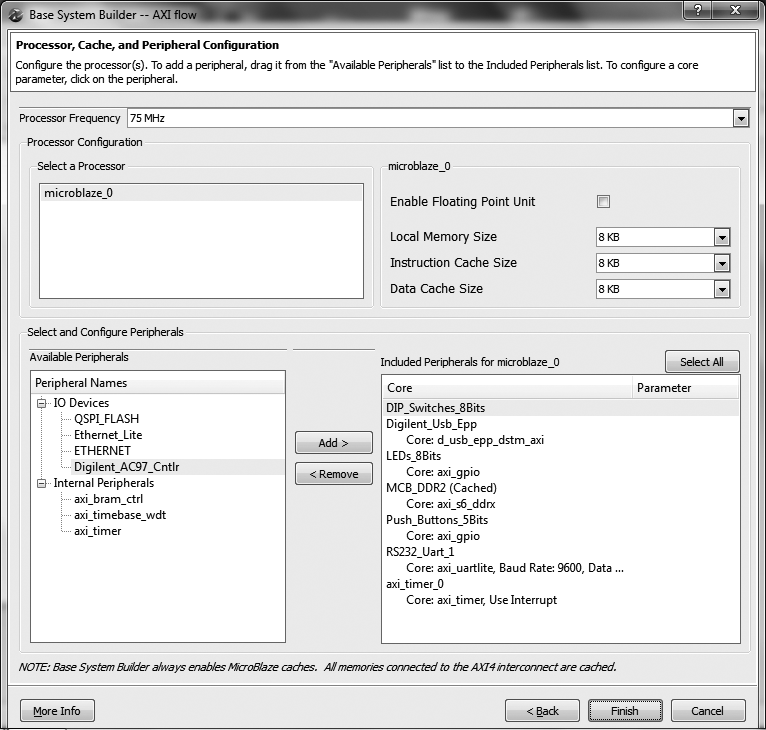
\includegraphics[width=0.65\linewidth,keepaspectratio]{./apendices/nuevos_proyectos_XPS/img/proyecto05}
		\caption{Ventana de configuraci�n del MicroBlaze del asistente de creaci�n de proyectos del XPS}
		\label{fig:proyecto05}
	\end{figure}
	
	Haciendo click en \emph{Finish} se finalizar� este asistente y dar� paso a la siguiente ventana.
	
	\begin{figure}[H]
		\centering
		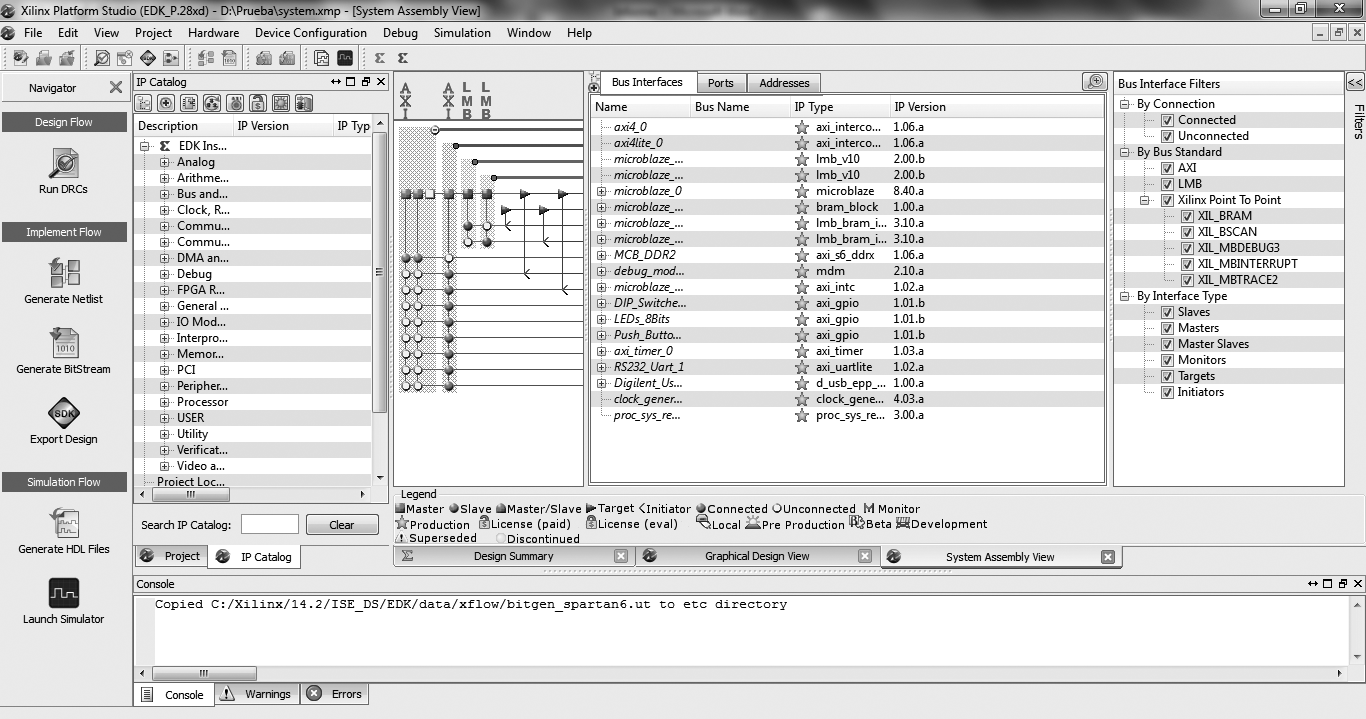
\includegraphics[width=0.6\linewidth,keepaspectratio]{./apendices/nuevos_proyectos_XPS/img/proyecto06}
		\caption{Ventana principal de trabajo del XPS}
		\label{fig:proyecto06}
	\end{figure}
	
	La ventana anterior (Figura \ref{fig:proyecto06}), muestra cada componente del sistema y sus conexiones. La 
	Figura siguiente (\ref{fig:proyecto07}) mostrar� esto con mayor detalle.
	
	\begin{figure}[H]
		\centering
		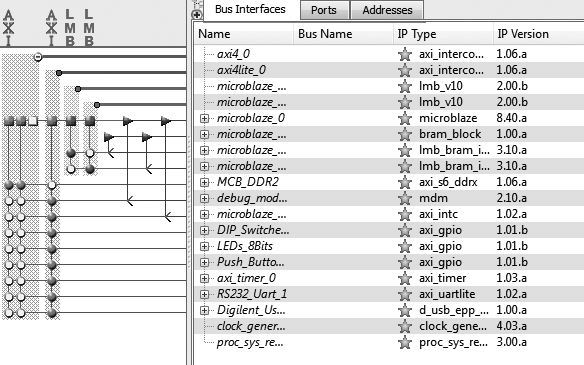
\includegraphics[width=1\linewidth,keepaspectratio]{./apendices/nuevos_proyectos_XPS/img/proyecto07}
		\caption{Ventana principal de trabajo del XPS}
		\label{fig:proyecto07}
	\end{figure}
	
	Para mayor informaci�n sobre este proceso, es posible encontrar manuales de referencia, tutoriales y ejemplos 
	en el sitio web de la empresa \emph{Xilinx}\footnote{\url{http://www.xilinx.com/}}